%==================================================== 
% Document Settings
\documentclass[a4paper,12pt]{article}
\usepackage[utf8]{inputenc}
\usepackage{graphicx}
\usepackage{amsmath}
\usepackage[table]{xcolor}
\usepackage{multirow}
\usepackage{geometry}
 \geometry{
 a4paper,
 left=40mm,
 right=30mm,
 top=30mm,
 bottom=30mm,
 }
% \usepackage{showframe}
%==================================================== 
% Document Owners
\title{}
\author{}
\date{}

\pdfinfo{%
  /Title    (Proposal Tugas Akhir)
  /Author   (Achmadi)
  /Creator  (Achmadi)
  /Producer (Achmadi)
  /Subject  (Buat TA)
  /Keywords (TA dan TA)
}
%==================================================== 
% Document Content
\begin{document}
\pagenumbering{gobble}
%==================================================== 
% Cover
\begin{center}
  \textbf{ \Large{PROPOSAL TUGAS AKHIR } }\\[5pt]
  \textbf{ \large{Rancang Bangun \textit{Robot Vision} Menggunakan \textit{Color Tracking} pada perangkat RaspberryPi } }
  \\[50pt]
  
\includegraphics[width=200pt]{ITS}
  \\[50pt]
  \textbf{ \large{Disusun Oleh:} }\\
  \underline{\textbf{ \large{Achmadi} } }\\
  \textbf{ \large{NRP: 2410100085 } }\\[40pt]
  \textbf{ \large{Pembimbing: } }\\
  \textbf{ \large{Ir. Apriani K. MSc \hspace{50pt} NIP: 195304041979012001} }\\[60pt]
  \textbf{ \large{PROGRAM STUDI S-1 TEKNIK FISIKA } }\\
  \textbf{ \large{JURUSAN TEKNIK FISIKA } }\\
  \textbf{ \large{FAKULTAS TEKNOLOGI INDUSTRI } }\\
  \textbf{ \large{INSTITUT TEKNOLOGI SEPULUH NOPEMBER } }\\
  \textbf{ \large{SURABAYA } }\\
  \textbf{ \large{2014 } }\\
\end{center}
%==================================================== 
% Pengesahan
\newpage
\begin{center}
  \textbf{ LEMBAR PENGESAHAN  }\\[5pt]
  \textbf{ PROPOSAL TUGAS AKHIR  } \\[5pt]
  \textbf{ JURUSAN TEKNIK FISIKA FTI-ITS  }\\[5pt]
\end{center}
\rule{385pt}{5pt}\\
\noindent Judul \hspace{80pt} : Rancang Bangun \textit{Robot Vision} Menggunakan \textit{Color Tracking} pada perangkat RaspberryPi\\[5pt]
\noindent Bidang Studi \hspace{42pt} : Rekayasa Fotonika\\[5pt]
\noindent 1. Nama Mahasiswa \hspace{5pt} : Achmadi\\[5pt]
\noindent 2. NRP  \hspace{70pt} : 2410100085\\[5pt]
\noindent 3. Jangka Waktu \hspace{20pt} : 3 bulan (Oktober-Desember)\\[5pt]
\noindent 4. Pembimbing \hspace{28pt} : Ir. Apriani K. MSc\\[5pt]
\noindent 5. Usulan ke \hspace{40pt} : 1\\[5pt]
\noindent 6. Status \hspace{60pt} : Baru\\[5pt]
\rule{385pt}{5pt}
\begin{flushright}
  Surabaya, 15 September 2014
\end{flushright}
\begin{flushleft}
Pembimbing, \hspace{230pt} Pengusul, 
\\[40pt]
\underline{Ir. Apriani K. MSc} \hspace{200pt} \underline{Achmadi}\\
NIP: 195304041979012001 \hspace{150pt} NRP: 2410100085
\\[40pt]
\end{flushleft}
\begin{center}
  Mengetahui,\\
  Kepala Laboratorium Rekayasa Fotonika
  \\[40pt]
  \underline{Prof. Dr, Ir. Sekartedjo M.Sc}\\
  NIP. 195004021979011001
\end{center}
\newpage
\begin{center}
 \textbf{PROPOSAL TUGAS AKHIR}
\end{center}
%==================================================== 
% Pendahuluan
\noindent \textbf{I. \hspace{10pt} Judul}

Rancang Bangun \textit{Robot Vision} Menggunakan \textit{Color Tracking} pada perang-\ kat RaspberryPi
\\[10pt]
\noindent \textbf{II. \hspace{9pt} Mata Kuliah Pilihan Bidang Minat Yang Diambil}

1. Pengolahan Citra

2. Metrologi Optik
\\[10pt]
\noindent \textbf{III. \hspace{8pt} Pembimbing}

1. Ir. Apriani K. MSc
\\[10pt]
\noindent \textbf{IV. \hspace{9pt} Latar Belakang} 

Robot vision adalah robot yang mampu menggunakan kamera sebagai sumber informasi untuk diolah sesuai kebutuhan \cite{robot}.
Tujuan utama setiap perancangan robot tentu adalah untuk mengganti pekerjaan manusia.
Kemampuan robot untuk melakukan pekerjaan yang berulang dan berbahaya telah menjadi kebutuhan di setiap lingkungan industri \cite{robot_function} . 
Untuk memenuhi kebutuhan tersebut telah dikembangkan beragam teknologi sensor dan actuator.
Khusus untuk sensor, telah dikembangkan teknologi yang mirip dengan cara kerja pada indra manusia.
Salah satu yang banyak dipakai adalah penggunaan kamera sebagai pengganti mata untuk robot \cite{robot}.

Penggunaan kamera sebagai sensor visual telah banyak di terapkan pada bidang robotika \cite{robot}.
Sebagai contoh robot Asimo dengan harga \$2.500.000 per unit menggunakan kamera CCD diproses dengan 20 CPU buatan Honda \cite{asimo}.
Kemudian robot Noa dengan harga \$7.900 per unit menggunakan kamera SOC yang diproses dengan Intel Atom \cite{nao}.
Sedangkan robot Darwin-Op dengan harga \$12.000 per unit menggunakan kamera CMOS diproses dengan Intel Atom \cite{darwinop}.
Berdasarkan informasi tersebut, maka harga tersebut masih tergolong mahal untuk aplikasi skala rumah dan kantor secara umum.

RaspberryPi merupakan salah satu jenis SBC (Single Board Computer) dengan spesifikasi processor BCM235 arsitektur arm1176 kategori armhf dan RAM 512.
Tersedia Operating System yang dapat dijalankan oleh RaspberryPi yaitu Raspbian yang berbasis Linux dan memiliki pustaka pengolahan citra OpenCV di lumbung perangkat lunaknya.
RaspberryPi dan Operating System Raspbian merupakan proyek opensource yang bersifat gratis \cite{raspi}.
Perangkat RaspberryPi tersedia dengan harga cukup murah yaitu hanya \$60 dan memiliki antar muka USB sehingga dapat berkomunikasi dengan kamera webcam.

Pustaka OpenCV (Open Computer Vision) merupakan pustaka pemrograman berbasis C/C++ yang berisi fungsi-fungsi untuk akuisisi dan pengolahan citra.
Pustaka OpenCV juga merupakan proyek opensource yang bersifat gratis.
Saat ini pustaka OpenCV telah diterapkan di banyak website dan aplikasi mobile untuk deteksi wajah dan penjejak warna \cite{opencv_intro}.
Penjejakan warna merupakan salah satu bentuk pengenalan objek yang cukup sederhana. 
Prinsip proses penjejakan warna adalah mensegmentasi gambar sesuai warna kemudian membaca perubahan koordinat warna yang tidak tersegmentasi relatif terhadap dimensi gambar.
Prinsip penjejakan warna ini dapat digunakan untuk mengenali suatu objek dan membuang objek lain sesuai warna kemudian mengikuti perubahan pixel warna yang tidak tersegmentasi untuk mengetahui perubahan posisi objek yang dikenali.
\\[10pt]
\noindent \textbf{V. \hspace{10pt} Rumusan Masalah}

Berdasarkan latar belakang di atas, permasalahan yang akan diangkat adalah bagaimana merancang bangun robot vision berbasis color tracking menggunakan OpenCV pada perangkat RaspberryPi.
\\[10pt]
\noindent \textbf{VI. \hspace{9pt} Tujuan}

Tujuan dari tugas akhir ini adalah merancang bangun robot vision berbasis color tracking menggunakan OpenCV pada perangkat RaspberryPi.
\\[10pt]
\noindent \textbf{VII. \hspace{8pt} Batasan Masalah}

Penelitian tugas akhir ini dibatasi pada kajian rancang bangun robot yang menggunakan kamera dan pengolahan citra untuk mengenali dan mengikuti objek berdasarkan warna yang dimiliki objek tersebut.
\\[10pt]
\noindent \textbf{VIII. \hspace{7pt} Teori Penunjang}

\indent \textbf{8.1. \hspace{8pt} Mode Warna HSV}

Dalam pengolahan citra, dikenal mode warna sebagai representasi cara manusia melihat \cite{robot} . 
Mode warna yang banyak digunakan adalah RGB, CMYK, HSL, dan HSV \cite{improc1}. 
Mode warna HSV adalah mode warna yang menyatakan warna dalam 3 variabel yaitu Hue, Saturation, dan Value.

Nilai Hue merepresentasikan nilai jenis warna yang merupakan nilai kombinasi RGB dalam besaran sudut. 
Pada dasarnya nilai Hue dibagi dalam juring lingkaran sehingga jangkauan nilainya adalah 0-360, namun karena dalam bahasa pemrograman variabel pemrograman hanya 8bit (0-255) maka jangkauan juring di reduksi menjadi setengah lingkaran (0-179) \cite{opencv_intro}.

Untuk lingkaran penuh, maka nilai Hue dapat direpresentasikan seperti berikut:
\begin{center}
 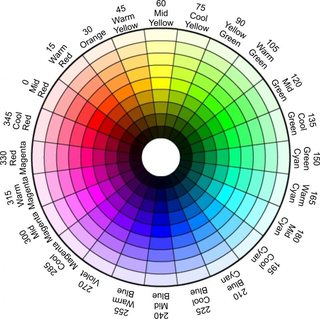
\includegraphics[width=200pt]{HSV}
\end{center}

Grafik di atas dibentuk dari perpaduan RGB dengan masing-masing nilai R, G, dan B terpisah sejauh 120 derajat.
Maka nilai warna lain merupakan perpaduan dua warna dalam rentang 120 derajat tersebut.

Sedangkan untuk dapat diolah dalam variabel 8 bit, maka nilai sudut di atas dibagi 2, sehingga nilai Hue terbagi menjadi 180 nilai (0-179) dengan rincian sebagai berikut:\\
1. Oranye (0-22)\\
2. Kuning (22-38)\\
3. Hijau (38-75)\\
4. Biru (75-130)\\
5. Ungu (130-160)\\
6. Merah (160-179)

Nilai Saturation merepresentasikan tingkat campuran suatu warna dengan warna putih dengan jangkauan nilai 0-255.
Sedangkan nilai Value merepresentasikan tingkat campuran suatu warna dengan warna hitam dengan jangkauan nilai 0-255.
Nilai Saturation dan Value sangat terpengaruh oleh tingkat pencahayaan \cite{opencv_intro} .

Pustaka OpenCV telah menyediakan fungsi untuk konversi RGB ke HSV.
Konversi ini diperlukan karena hasil output kamera adalah matriks RGB sedangkan pengolahan selanjutnya menggunakan HSV.

Dalam konversi RGB ke HSV, nilai V didapat dari nilai terbesar di antara nilai R, G, dan B. 
Secara matematis dinyatakan dengan:

\begin{equation}
  V = max(R,G,B)
\end{equation}

Untuk nilai S didapat dari rasio antara selisih V dikurangi nilai minimal di antara R, G, dan B dibandingkan dengan nilai V itu sendiri.
Secara matematis dinyatakan dengan:

\begin{equation}
  S =  
  \begin{cases}
      \frac{V-min(R,G,B)}{V},& \text{jika } V\neq 0\\
      0,              & \text{jika } V = 0\\
  \end{cases}
\end{equation}


Sedangkan untuk nilai Hue, maka konversi nilai RGB ke Hue dalam nilai bentuk sudut dinyatakan sebagai:

\begin{equation}
  H =  
  \begin{cases}
      \frac{60(G-B)}{(V-min(R,G,B))},& \text{jika } V = R\\
      120 + \frac{60(B-R)}{(V-min(R,G,B))},& \text{jika } V = G\\
      240 + \frac{60(R-G)}{(V-min(R,G,B))},& \text{jika } V = B\\
  \end{cases}
\end{equation}

Konversi di atas menggunakan 360 derajat.
Dalam pemrograman bilangan 8 bit hanya maximal 255 maka nilai 360 dibagi 2 sehingga kisaran nilai menjadi 0-179.
\\[10pt]
\indent \textbf{8.2. \hspace{8pt} Segmentasi Citra}

Segmentasi citra adalah proses mengumpulkan pixel-pixel karena kesamaan properti.
Kesamaan properti dapat berupa nilai intensitas, bentuk tekstur, garis tepi, dll.
Ada banyak teknik untuk segmentasi citra dengan masing-masing memiliki kompleksitas, kemampuan, dan penggunaannya.

Proses segmentasi merupakan proses yang penting dalam pengolahan citra.
Segmentasi digunakan untuk memfilter objek yang tidak dibutuhkan.
Filter dapat berupa persamaan matematis,logic maupun maupun matrix kernel \cite{improc1} .
\\[10pt]
\noindent \textbf{IX. \hspace{9pt} Metodologi Penelitian}

Pada penelitian tugas akhir ini langkah awal yang dilakukan adalah studi literatur.
Studi literatur ini digunakan untuk mendapatkan referensi mengenai skema peralatan dan perancangan eksperimen yang sesuai.
Langkah kedua adalah pembuatan robot berdasarkan literatur atau design yang telah ada.
Langkah ketiga adalah menguji robot untuk mendapatkan data performa robot tersebut pada variasi tingkat pencahayaan.
Langkah keempat adalah membuat analisis mengenai hasil yang diperoleh dari eksperimen. 
Selanjutnya langkah terakhir adalah penulisan laporan.

Berikut flowchart dari penelitian yang akan dilakukan:

\begin{center}
 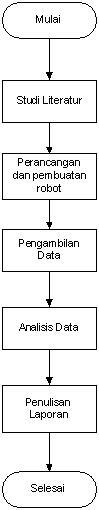
\includegraphics[height=450pt]{flow}
\end{center}

\vspace{40pt}

Berikut skema awal dari robot vision yang akan dibuat:

\begin{center}
 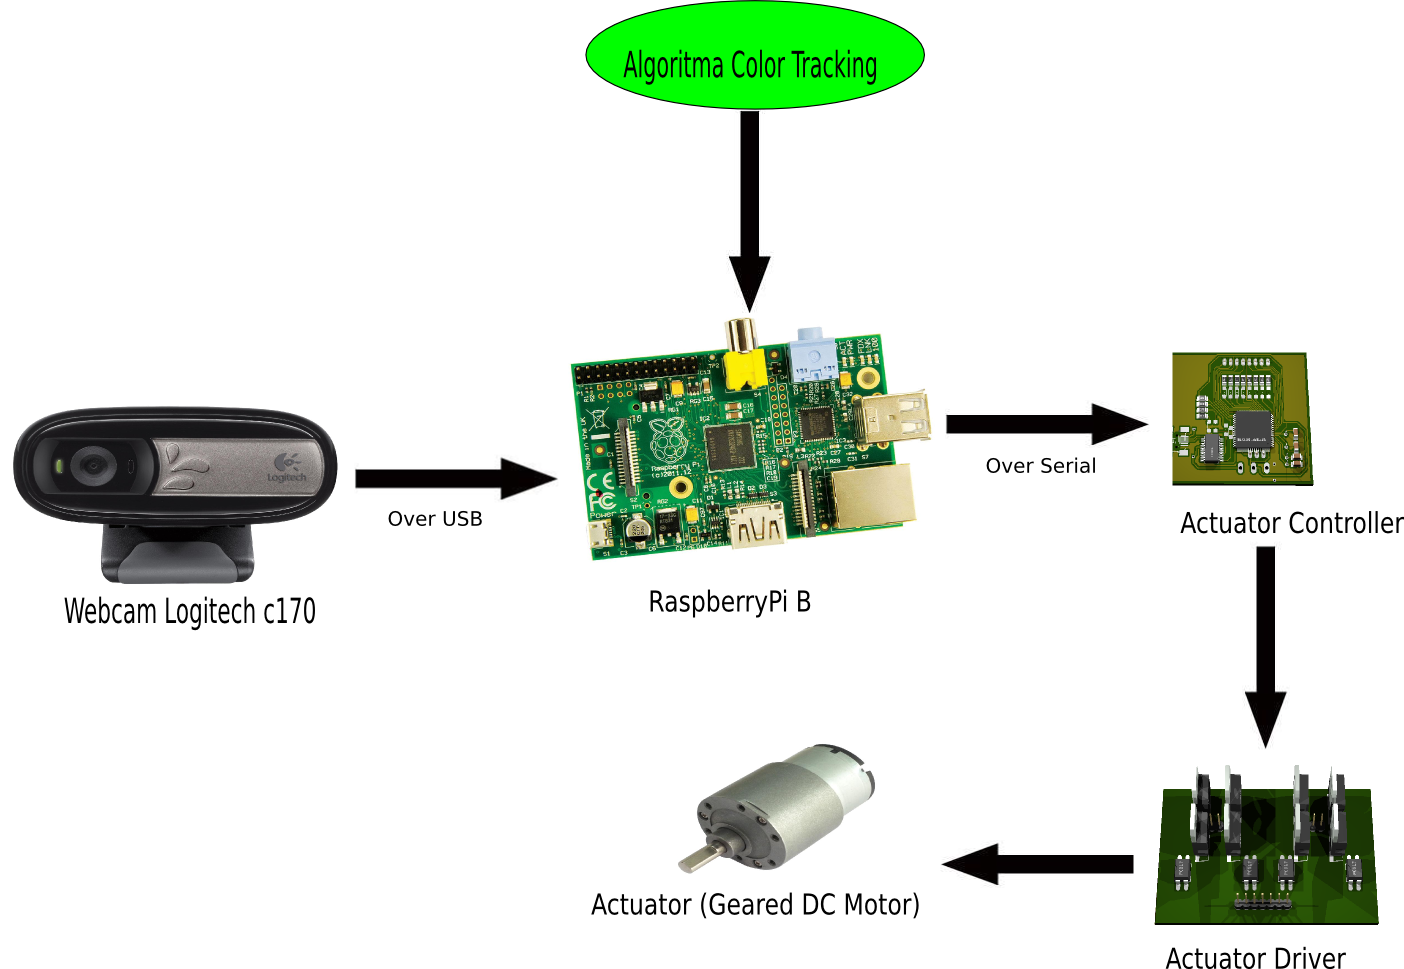
\includegraphics[width=350pt]{desain_awal}
\end{center}

\vspace{10pt}
\noindent \textbf{IX. \hspace{9pt} Jadwal Kerja}

Jadwal penelitian yang akan dilakukan tertera pada tabel di bawah ini.

\begin{center}
 \begin{tabular}{ |l|l|l|l|l|l| }
   \hline
   No & Kegiatan & \multicolumn{3}{|c|}{Bulan} \\
   \hline
     &  & 1 & 2 & 3 \\
   \hline
   1 & Studi literatur & \cellcolor{blue} & & \\
   \hline
   2 & Perancangan dan Pembuatan & \cellcolor{blue} & & \\
   \hline
   3 & Pengambilan Data & & \cellcolor{blue} & \\
   \hline
   4 & Analisa Data & & & \cellcolor{blue} \\
   \hline
   5 & Penulisan Laporan & & \cellcolor{blue} & \cellcolor{blue} \\
  \hline
\end{tabular}
\end{center}

\vspace{10pt}
\noindent \textbf{X. \hspace{9pt} Daftar Pustaka} 

\begingroup
  \renewcommand{\section}[2]{}%
    \begin{thebibliography}{}
	\bibitem{robot} Browning, Brett \textit{Real-Time, Adaptive Color-based Robot Vision} 2013
	\bibitem{robot_function} Chao, Fei \textit{A developmental approach to robotic pointing via human–robot interaction} 2014
	\bibitem{asimo} Honda Team \textit{Asimo Technical Information} 2007
	\bibitem{nao} Aldebaran Robotics \textit{Nao Technical Datasheet} 2012
	\bibitem{darwinop} Robotis \textit{Darwin-Op Technical Manual} 2012
	\bibitem{raspi} Upton, Eben \textit{RaspberryPi User Guide} 2012
	\bibitem{opencv_intro} OpenCV Team \textit{The OpenCV Reference Manual} 2014
	\bibitem{hsv} Phillips, Dwyne \textit{Image Processing in C} 2000
	\bibitem{improc1} Zhou, Huiyu \textit{Digital Image Processing Part I} 2010
    \end{thebibliography}
\endgroup

\end{document}
